% Options for packages loaded elsewhere
\PassOptionsToPackage{unicode}{hyperref}
\PassOptionsToPackage{hyphens}{url}
\PassOptionsToPackage{dvipsnames,svgnames,x11names}{xcolor}
%
\documentclass[
]{article}
\usepackage{amsmath,amssymb}
\usepackage{lmodern}
\usepackage{iftex}
\ifPDFTeX
  \usepackage[T1]{fontenc}
  \usepackage[utf8]{inputenc}
  \usepackage{textcomp} % provide euro and other symbols
\else % if luatex or xetex
  \usepackage{unicode-math}
  \defaultfontfeatures{Scale=MatchLowercase}
  \defaultfontfeatures[\rmfamily]{Ligatures=TeX,Scale=1}
\fi
% Use upquote if available, for straight quotes in verbatim environments
\IfFileExists{upquote.sty}{\usepackage{upquote}}{}
\IfFileExists{microtype.sty}{% use microtype if available
  \usepackage[]{microtype}
  \UseMicrotypeSet[protrusion]{basicmath} % disable protrusion for tt fonts
}{}
\makeatletter
\@ifundefined{KOMAClassName}{% if non-KOMA class
  \IfFileExists{parskip.sty}{%
    \usepackage{parskip}
  }{% else
    \setlength{\parindent}{0pt}
    \setlength{\parskip}{6pt plus 2pt minus 1pt}}
}{% if KOMA class
  \KOMAoptions{parskip=half}}
\makeatother
\usepackage{xcolor}
\usepackage[margin=1in]{geometry}
\usepackage{color}
\usepackage{fancyvrb}
\newcommand{\VerbBar}{|}
\newcommand{\VERB}{\Verb[commandchars=\\\{\}]}
\DefineVerbatimEnvironment{Highlighting}{Verbatim}{commandchars=\\\{\}}
% Add ',fontsize=\small' for more characters per line
\usepackage{framed}
\definecolor{shadecolor}{RGB}{248,248,248}
\newenvironment{Shaded}{\begin{snugshade}}{\end{snugshade}}
\newcommand{\AlertTok}[1]{\textcolor[rgb]{0.94,0.16,0.16}{#1}}
\newcommand{\AnnotationTok}[1]{\textcolor[rgb]{0.56,0.35,0.01}{\textbf{\textit{#1}}}}
\newcommand{\AttributeTok}[1]{\textcolor[rgb]{0.77,0.63,0.00}{#1}}
\newcommand{\BaseNTok}[1]{\textcolor[rgb]{0.00,0.00,0.81}{#1}}
\newcommand{\BuiltInTok}[1]{#1}
\newcommand{\CharTok}[1]{\textcolor[rgb]{0.31,0.60,0.02}{#1}}
\newcommand{\CommentTok}[1]{\textcolor[rgb]{0.56,0.35,0.01}{\textit{#1}}}
\newcommand{\CommentVarTok}[1]{\textcolor[rgb]{0.56,0.35,0.01}{\textbf{\textit{#1}}}}
\newcommand{\ConstantTok}[1]{\textcolor[rgb]{0.00,0.00,0.00}{#1}}
\newcommand{\ControlFlowTok}[1]{\textcolor[rgb]{0.13,0.29,0.53}{\textbf{#1}}}
\newcommand{\DataTypeTok}[1]{\textcolor[rgb]{0.13,0.29,0.53}{#1}}
\newcommand{\DecValTok}[1]{\textcolor[rgb]{0.00,0.00,0.81}{#1}}
\newcommand{\DocumentationTok}[1]{\textcolor[rgb]{0.56,0.35,0.01}{\textbf{\textit{#1}}}}
\newcommand{\ErrorTok}[1]{\textcolor[rgb]{0.64,0.00,0.00}{\textbf{#1}}}
\newcommand{\ExtensionTok}[1]{#1}
\newcommand{\FloatTok}[1]{\textcolor[rgb]{0.00,0.00,0.81}{#1}}
\newcommand{\FunctionTok}[1]{\textcolor[rgb]{0.00,0.00,0.00}{#1}}
\newcommand{\ImportTok}[1]{#1}
\newcommand{\InformationTok}[1]{\textcolor[rgb]{0.56,0.35,0.01}{\textbf{\textit{#1}}}}
\newcommand{\KeywordTok}[1]{\textcolor[rgb]{0.13,0.29,0.53}{\textbf{#1}}}
\newcommand{\NormalTok}[1]{#1}
\newcommand{\OperatorTok}[1]{\textcolor[rgb]{0.81,0.36,0.00}{\textbf{#1}}}
\newcommand{\OtherTok}[1]{\textcolor[rgb]{0.56,0.35,0.01}{#1}}
\newcommand{\PreprocessorTok}[1]{\textcolor[rgb]{0.56,0.35,0.01}{\textit{#1}}}
\newcommand{\RegionMarkerTok}[1]{#1}
\newcommand{\SpecialCharTok}[1]{\textcolor[rgb]{0.00,0.00,0.00}{#1}}
\newcommand{\SpecialStringTok}[1]{\textcolor[rgb]{0.31,0.60,0.02}{#1}}
\newcommand{\StringTok}[1]{\textcolor[rgb]{0.31,0.60,0.02}{#1}}
\newcommand{\VariableTok}[1]{\textcolor[rgb]{0.00,0.00,0.00}{#1}}
\newcommand{\VerbatimStringTok}[1]{\textcolor[rgb]{0.31,0.60,0.02}{#1}}
\newcommand{\WarningTok}[1]{\textcolor[rgb]{0.56,0.35,0.01}{\textbf{\textit{#1}}}}
\usepackage{graphicx}
\makeatletter
\def\maxwidth{\ifdim\Gin@nat@width>\linewidth\linewidth\else\Gin@nat@width\fi}
\def\maxheight{\ifdim\Gin@nat@height>\textheight\textheight\else\Gin@nat@height\fi}
\makeatother
% Scale images if necessary, so that they will not overflow the page
% margins by default, and it is still possible to overwrite the defaults
% using explicit options in \includegraphics[width, height, ...]{}
\setkeys{Gin}{width=\maxwidth,height=\maxheight,keepaspectratio}
% Set default figure placement to htbp
\makeatletter
\def\fps@figure{htbp}
\makeatother
\setlength{\emergencystretch}{3em} % prevent overfull lines
\providecommand{\tightlist}{%
  \setlength{\itemsep}{0pt}\setlength{\parskip}{0pt}}
\setcounter{secnumdepth}{-\maxdimen} % remove section numbering
\ifLuaTeX
  \usepackage{selnolig}  % disable illegal ligatures
\fi
\IfFileExists{bookmark.sty}{\usepackage{bookmark}}{\usepackage{hyperref}}
\IfFileExists{xurl.sty}{\usepackage{xurl}}{} % add URL line breaks if available
\urlstyle{same} % disable monospaced font for URLs
\hypersetup{
  pdftitle={36-315 Final Project Data Pre-analysis},
  pdfauthor={Arthur Jakobsson, Alex Cheng, Liz Chu, Kevin Ren},
  colorlinks=true,
  linkcolor={Maroon},
  filecolor={Maroon},
  citecolor={Blue},
  urlcolor={blue},
  pdfcreator={LaTeX via pandoc}}

\title{36-315 Final Project Data Pre-analysis}
\author{Arthur Jakobsson, Alex Cheng, Liz Chu, Kevin Ren}
\date{November 18, 2022}

\begin{document}
\maketitle

{
\hypersetup{linkcolor=}
\setcounter{tocdepth}{2}
\tableofcontents
}
\hypertarget{rat-sighting-dataset---data-pre-analysis}{%
\section{Rat Sighting Dataset - Data
Pre-analysis}\label{rat-sighting-dataset---data-pre-analysis}}

\begin{Shaded}
\begin{Highlighting}[]
\CommentTok{\# library imports}

\FunctionTok{library}\NormalTok{(tigris)}
\end{Highlighting}
\end{Shaded}

\begin{verbatim}
## To enable caching of data, set `options(tigris_use_cache = TRUE)`
## in your R script or .Rprofile.
\end{verbatim}

\begin{Shaded}
\begin{Highlighting}[]
\FunctionTok{library}\NormalTok{(dplyr)}
\end{Highlighting}
\end{Shaded}

\begin{verbatim}
## 
## Attaching package: 'dplyr'
\end{verbatim}

\begin{verbatim}
## The following objects are masked from 'package:stats':
## 
##     filter, lag
\end{verbatim}

\begin{verbatim}
## The following objects are masked from 'package:base':
## 
##     intersect, setdiff, setequal, union
\end{verbatim}

\begin{Shaded}
\begin{Highlighting}[]
\FunctionTok{library}\NormalTok{(leaflet)}
\FunctionTok{library}\NormalTok{(tidyverse)}
\end{Highlighting}
\end{Shaded}

\begin{verbatim}
## -- Attaching packages --------------------------------------- tidyverse 1.3.2 --
\end{verbatim}

\begin{verbatim}
## v ggplot2 3.4.0     v purrr   0.3.5
## v tibble  3.1.8     v stringr 1.4.1
## v tidyr   1.2.1     v forcats 0.5.2
## v readr   2.1.3     
## -- Conflicts ------------------------------------------ tidyverse_conflicts() --
## x dplyr::filter() masks stats::filter()
## x dplyr::lag()    masks stats::lag()
\end{verbatim}

\begin{Shaded}
\begin{Highlighting}[]
\FunctionTok{library}\NormalTok{(sp)}
\FunctionTok{library}\NormalTok{(ggmap)}
\end{Highlighting}
\end{Shaded}

\begin{verbatim}
## i Google's Terms of Service: <]8;;https://mapsplatform.google.comhttps://mapsplatform.google.com]8;;>
## i Please cite ggmap if you use it! Use `citation("ggmap")` for details.
\end{verbatim}

\begin{Shaded}
\begin{Highlighting}[]
\FunctionTok{library}\NormalTok{(maptools)}
\end{Highlighting}
\end{Shaded}

\begin{verbatim}
## Checking rgeos availability: TRUE
## Please note that 'maptools' will be retired during 2023,
## plan transition at your earliest convenience;
## some functionality will be moved to 'sp'.
\end{verbatim}

\begin{Shaded}
\begin{Highlighting}[]
\FunctionTok{library}\NormalTok{(broom)}
\FunctionTok{library}\NormalTok{(httr)}
\FunctionTok{library}\NormalTok{(rgdal)}
\end{Highlighting}
\end{Shaded}

\begin{verbatim}
## Please note that rgdal will be retired during 2023,
## plan transition to sf/stars/terra functions using GDAL and PROJ
## at your earliest convenience.
## See https://r-spatial.org/r/2022/04/12/evolution.html and https://github.com/r-spatial/evolution
## rgdal: version: 1.6-2, (SVN revision 1183)
## Geospatial Data Abstraction Library extensions to R successfully loaded
## Loaded GDAL runtime: GDAL 3.5.3, released 2022/10/21
## Path to GDAL shared files: /Library/Frameworks/R.framework/Versions/4.2-arm64/Resources/library/sf/gdal
##  GDAL does not use iconv for recoding strings.
## GDAL binary built with GEOS: TRUE 
## Loaded PROJ runtime: Rel. 9.1.0, September 1st, 2022, [PJ_VERSION: 910]
## Path to PROJ shared files: /Library/Frameworks/R.framework/Versions/4.2-arm64/Resources/library/rgdal/proj
## PROJ CDN enabled: FALSE
## Linking to sp version:1.5-1
## To mute warnings of possible GDAL/OSR exportToProj4() degradation,
## use options("rgdal_show_exportToProj4_warnings"="none") before loading sp or rgdal.
\end{verbatim}

\begin{Shaded}
\begin{Highlighting}[]
\FunctionTok{library}\NormalTok{(gridExtra)}
\end{Highlighting}
\end{Shaded}

\begin{verbatim}
## 
## Attaching package: 'gridExtra'
## 
## The following object is masked from 'package:dplyr':
## 
##     combine
\end{verbatim}

\begin{Shaded}
\begin{Highlighting}[]
\FunctionTok{library}\NormalTok{(stringr)}
\FunctionTok{library}\NormalTok{(geosphere)}
\CommentTok{\# distm(c(lon1, lat1), c(lon2, lat2), fun = distHaversine)}
\end{Highlighting}
\end{Shaded}

\begin{Shaded}
\begin{Highlighting}[]
\CommentTok{\# maps setup}

\CommentTok{\#nice map (manhattan, brooklyn, queens, a bit of bronx)}
\NormalTok{left }\OtherTok{=}\SpecialCharTok{{-}}\FloatTok{74.03} 
\NormalTok{bottom }\OtherTok{=} \FloatTok{40.68} 
\NormalTok{right }\OtherTok{=} \SpecialCharTok{{-}}\FloatTok{73.87}
\NormalTok{top }\OtherTok{=} \FloatTok{40.85}
\NormalTok{nyc\_coords }\OtherTok{\textless{}{-}} \FunctionTok{c}\NormalTok{(left, bottom, right, top)}

\CommentTok{\#full map (all boroughs)}
\NormalTok{leftF }\OtherTok{=} \SpecialCharTok{{-}}\FloatTok{74.2}
\NormalTok{bottomF }\OtherTok{=} \FloatTok{40.55}
\NormalTok{rightF }\OtherTok{=} \SpecialCharTok{{-}}\FloatTok{73.87}
\NormalTok{topF }\OtherTok{=} \FloatTok{40.85}
\NormalTok{nyc\_coordsF }\OtherTok{\textless{}{-}} \FunctionTok{c}\NormalTok{(leftF, bottomF, rightF, topF)}

\CommentTok{\#just dowtown manhattan}
\NormalTok{leftM }\OtherTok{=} \SpecialCharTok{{-}}\FloatTok{74.03}
\NormalTok{bottomM }\OtherTok{=} \FloatTok{40.69}
\NormalTok{rightM }\OtherTok{=} \SpecialCharTok{{-}}\FloatTok{73.94}
\NormalTok{topM }\OtherTok{=} \FloatTok{40.81}
\NormalTok{nyc\_coordsM }\OtherTok{\textless{}{-}} \FunctionTok{c}\NormalTok{(leftM, bottomM, rightM, topM)}

\NormalTok{nyc\_map }\OtherTok{\textless{}{-}} \FunctionTok{get\_stamenmap}\NormalTok{(nyc\_coords, }\AttributeTok{maptype =} \StringTok{"terrain"}\NormalTok{, }\AttributeTok{zoom =} \DecValTok{11}\NormalTok{)}
\end{Highlighting}
\end{Shaded}

\begin{verbatim}
## i Map tiles by Stamen Design, under CC BY 3.0. Data by OpenStreetMap, under ODbL.
\end{verbatim}

\begin{Shaded}
\begin{Highlighting}[]
\NormalTok{nyc\_mapF }\OtherTok{\textless{}{-}} \FunctionTok{get\_stamenmap}\NormalTok{(nyc\_coordsF, }\AttributeTok{maptype =} \StringTok{"terrain"}\NormalTok{, }\AttributeTok{zoom =} \DecValTok{11}\NormalTok{)}
\end{Highlighting}
\end{Shaded}

\begin{verbatim}
## i Map tiles by Stamen Design, under CC BY 3.0. Data by OpenStreetMap, under ODbL.
\end{verbatim}

\begin{Shaded}
\begin{Highlighting}[]
\NormalTok{nyc\_mapM }\OtherTok{\textless{}{-}} \FunctionTok{get\_stamenmap}\NormalTok{(nyc\_coordsM, }\AttributeTok{maptype =} \StringTok{"terrain"}\NormalTok{, }\AttributeTok{zoom =} \DecValTok{11}\NormalTok{)}
\end{Highlighting}
\end{Shaded}

\begin{verbatim}
## i Map tiles by Stamen Design, under CC BY 3.0. Data by OpenStreetMap, under ODbL.
\end{verbatim}

\begin{Shaded}
\begin{Highlighting}[]
\NormalTok{nyc\_neighborhoods\_df }\OtherTok{\textless{}{-}} \FunctionTok{tidy}\NormalTok{(nyc\_neighborhoods) }\CommentTok{\# https://rpubs.com/jhofman/nycmaps}
\end{Highlighting}
\end{Shaded}

\begin{verbatim}
## Regions defined for each Polygons
\end{verbatim}

\begin{Shaded}
\begin{Highlighting}[]
\CommentTok{\# @here I tried to make this map larger but I couldn\textquotesingle{}t figure out how}
\NormalTok{nyc\_mapPolygon }\OtherTok{\textless{}{-}} \FunctionTok{ggmap}\NormalTok{(nyc\_map) }\SpecialCharTok{+}
  \FunctionTok{geom\_polygon}\NormalTok{(}\AttributeTok{data=}\NormalTok{nyc\_neighborhoods\_df, }\FunctionTok{aes}\NormalTok{(}\AttributeTok{x=}\NormalTok{long, }\AttributeTok{y=}\NormalTok{lat, }\AttributeTok{group=}\NormalTok{group), }\AttributeTok{color=}\StringTok{"blue"}\NormalTok{, }\AttributeTok{fill=}\ConstantTok{NA}\NormalTok{)}

\NormalTok{nyc\_mapFPolygon }\OtherTok{\textless{}{-}} \FunctionTok{ggmap}\NormalTok{(nyc\_mapF) }\SpecialCharTok{+}
  \FunctionTok{geom\_polygon}\NormalTok{(}\AttributeTok{data=}\NormalTok{nyc\_neighborhoods\_df, }\FunctionTok{aes}\NormalTok{(}\AttributeTok{x=}\NormalTok{long, }\AttributeTok{y=}\NormalTok{lat, }\AttributeTok{group=}\NormalTok{group), }\AttributeTok{color=}\StringTok{"blue"}\NormalTok{, }\AttributeTok{fill=}\ConstantTok{NA}\NormalTok{)}

\NormalTok{nyc\_mapMPolygon }\OtherTok{\textless{}{-}} \FunctionTok{ggmap}\NormalTok{(nyc\_mapM) }\SpecialCharTok{+} 
  \FunctionTok{geom\_polygon}\NormalTok{(}\AttributeTok{data=}\NormalTok{nyc\_neighborhoods\_df, }\FunctionTok{aes}\NormalTok{(}\AttributeTok{x=}\NormalTok{long, }\AttributeTok{y=}\NormalTok{lat, }\AttributeTok{group=}\NormalTok{group), }\AttributeTok{color=}\StringTok{"blue"}\NormalTok{, }\AttributeTok{fill=}\ConstantTok{NA}\NormalTok{)}

\CommentTok{\# nyc\_mapPolygon}
\CommentTok{\# nyc\_mapMPolygon}
\CommentTok{\# nyc\_mapFPolygon}
\end{Highlighting}
\end{Shaded}

\begin{Shaded}
\begin{Highlighting}[]
\CommentTok{\# importing rats}

\NormalTok{ratSubset }\OtherTok{\textless{}{-}} \FunctionTok{subset}\NormalTok{(rats, Longitude}\SpecialCharTok{\textless{}}\NormalTok{right }\SpecialCharTok{\&}\NormalTok{ Latitude}\SpecialCharTok{\textless{}}\NormalTok{top }\SpecialCharTok{\&}\NormalTok{ Longitude }\SpecialCharTok{\textgreater{}}\NormalTok{ left }\SpecialCharTok{\&}\NormalTok{ Latitude }\SpecialCharTok{\textgreater{}}\NormalTok{bottom)}
\NormalTok{ratSubsetF }\OtherTok{\textless{}{-}} \FunctionTok{subset}\NormalTok{(rats, Longitude}\SpecialCharTok{\textless{}}\NormalTok{rightF }\SpecialCharTok{\&}\NormalTok{ Latitude}\SpecialCharTok{\textless{}}\NormalTok{topF }\SpecialCharTok{\&}\NormalTok{ Longitude }\SpecialCharTok{\textgreater{}}\NormalTok{ leftF }\SpecialCharTok{\&}\NormalTok{ Latitude }\SpecialCharTok{\textgreater{}}\NormalTok{bottomF)}
\NormalTok{ratSubsetM }\OtherTok{\textless{}{-}} \FunctionTok{subset}\NormalTok{(rats, Longitude}\SpecialCharTok{\textless{}}\NormalTok{rightM }\SpecialCharTok{\&}\NormalTok{ Latitude}\SpecialCharTok{\textless{}}\NormalTok{topM }\SpecialCharTok{\&}\NormalTok{ Longitude }\SpecialCharTok{\textgreater{}}\NormalTok{ leftM }\SpecialCharTok{\&}\NormalTok{ Latitude }\SpecialCharTok{\textgreater{}}\NormalTok{bottomM)}

\NormalTok{health\_inspection[, }\FunctionTok{c}\NormalTok{(}\StringTok{"SCORE"}\NormalTok{)] }\OtherTok{\textless{}{-}} \FunctionTok{sapply}\NormalTok{(health\_inspection[, }\FunctionTok{c}\NormalTok{(}\StringTok{"SCORE"}\NormalTok{)], as.integer)}
\NormalTok{health\_inspection[}\StringTok{"SCORE"}\NormalTok{][}\FunctionTok{is.na}\NormalTok{(health\_inspection[}\StringTok{"SCORE"}\NormalTok{])] }\OtherTok{\textless{}{-}} \DecValTok{0}

\NormalTok{healthSubset }\OtherTok{\textless{}{-}} \FunctionTok{subset}\NormalTok{(health\_inspection, Longitude}\SpecialCharTok{\textless{}}\NormalTok{right }\SpecialCharTok{\&}\NormalTok{ Latitude}\SpecialCharTok{\textless{}}\NormalTok{top }\SpecialCharTok{\&}\NormalTok{ Longitude }\SpecialCharTok{\textgreater{}}\NormalTok{ left }\SpecialCharTok{\&}\NormalTok{ Latitude }\SpecialCharTok{\textgreater{}}\NormalTok{bottom }\SpecialCharTok{\&}\NormalTok{ SCORE}\SpecialCharTok{\textgreater{}}\DecValTok{50}\NormalTok{)}
\NormalTok{healthSubsetF }\OtherTok{\textless{}{-}} \FunctionTok{subset}\NormalTok{(health\_inspection, Longitude}\SpecialCharTok{\textless{}}\NormalTok{rightF }\SpecialCharTok{\&}\NormalTok{ Latitude}\SpecialCharTok{\textless{}}\NormalTok{topF }\SpecialCharTok{\&}\NormalTok{ Longitude }\SpecialCharTok{\textgreater{}}\NormalTok{ leftF }\SpecialCharTok{\&}\NormalTok{ Latitude }\SpecialCharTok{\textgreater{}}\NormalTok{bottomF }\SpecialCharTok{\&}\NormalTok{ SCORE}\SpecialCharTok{\textgreater{}}\DecValTok{50}\NormalTok{)}
\NormalTok{healthSubsetM }\OtherTok{\textless{}{-}} \FunctionTok{subset}\NormalTok{(health\_inspection, Longitude}\SpecialCharTok{\textless{}}\NormalTok{rightM }\SpecialCharTok{\&}\NormalTok{ Latitude}\SpecialCharTok{\textless{}}\NormalTok{topM }\SpecialCharTok{\&}\NormalTok{ Longitude }\SpecialCharTok{\textgreater{}}\NormalTok{ leftM }\SpecialCharTok{\&}\NormalTok{ Latitude }\SpecialCharTok{\textgreater{}}\NormalTok{bottomM }\SpecialCharTok{\&}\NormalTok{ SCORE}\SpecialCharTok{\textgreater{}}\DecValTok{50}\NormalTok{)}

\NormalTok{rat\_map }\OtherTok{\textless{}{-}} \FunctionTok{ggmap}\NormalTok{(nyc\_map) }\SpecialCharTok{+}
  \FunctionTok{geom\_point}\NormalTok{(}\AttributeTok{data=}\NormalTok{ratSubset, }\FunctionTok{aes}\NormalTok{(}\AttributeTok{x=}\NormalTok{Longitude, }\AttributeTok{y =}\NormalTok{ Latitude), }\AttributeTok{alpha=}\FloatTok{0.2}\NormalTok{, }\AttributeTok{size =}\FloatTok{0.01}\NormalTok{, }\AttributeTok{color =} \StringTok{"coral3"}\NormalTok{)}

\NormalTok{rat\_mapF }\OtherTok{\textless{}{-}} \FunctionTok{ggmap}\NormalTok{(nyc\_mapF) }\SpecialCharTok{+}
  \FunctionTok{geom\_point}\NormalTok{(}\AttributeTok{data=}\NormalTok{ratSubsetF, }\FunctionTok{aes}\NormalTok{(}\AttributeTok{x=}\NormalTok{Longitude, }\AttributeTok{y =}\NormalTok{ Latitude), }\AttributeTok{alpha=}\FloatTok{0.2}\NormalTok{, }\AttributeTok{size =}\FloatTok{0.01}\NormalTok{, }\AttributeTok{color =} \StringTok{"coral3"}\NormalTok{)}

\NormalTok{rat\_mapM }\OtherTok{\textless{}{-}} \FunctionTok{ggmap}\NormalTok{(nyc\_mapM) }\SpecialCharTok{+}
  \FunctionTok{geom\_point}\NormalTok{(}\AttributeTok{data=}\NormalTok{ratSubsetM, }\FunctionTok{aes}\NormalTok{(}\AttributeTok{x=}\NormalTok{Longitude, }\AttributeTok{y =}\NormalTok{ Latitude), }\AttributeTok{alpha=}\FloatTok{0.2}\NormalTok{, }\AttributeTok{size =}\FloatTok{0.01}\NormalTok{, }\AttributeTok{color =} \StringTok{"coral3"}\NormalTok{)}

\CommentTok{\# rat\_map}
\CommentTok{\# rat\_mapF}
\CommentTok{\# rat\_mapM}


\NormalTok{ratHealthScore\_map }\OtherTok{\textless{}{-}} \FunctionTok{ggmap}\NormalTok{(nyc\_map) }\SpecialCharTok{+}
  \FunctionTok{geom\_point}\NormalTok{(}\AttributeTok{data=}\NormalTok{ratSubset, }\FunctionTok{aes}\NormalTok{(}\AttributeTok{x=}\NormalTok{Longitude, }\AttributeTok{y =}\NormalTok{ Latitude), }\AttributeTok{alpha=}\FloatTok{0.2}\NormalTok{, }\AttributeTok{size =}\FloatTok{0.01}\NormalTok{, }\AttributeTok{color =} \StringTok{"chocolate3"}\NormalTok{)}\SpecialCharTok{+}
  \FunctionTok{geom\_point}\NormalTok{(}\AttributeTok{data=}\NormalTok{healthSubset, }\FunctionTok{aes}\NormalTok{(}\AttributeTok{x=}\NormalTok{Longitude, }\AttributeTok{y =}\NormalTok{ Latitude, }\AttributeTok{color =}\NormalTok{ SCORE), }\AttributeTok{size =} \FloatTok{0.5}\NormalTok{, }\AttributeTok{alpha=}\FloatTok{0.2}\NormalTok{) }\SpecialCharTok{+}
  \FunctionTok{scale\_color\_distiller}\NormalTok{(}\AttributeTok{palette =} \StringTok{"PiYG"}\NormalTok{)}

\NormalTok{ratHealthScore\_mapF }\OtherTok{\textless{}{-}} \FunctionTok{ggmap}\NormalTok{(nyc\_mapF) }\SpecialCharTok{+}
  \FunctionTok{geom\_point}\NormalTok{(}\AttributeTok{data=}\NormalTok{ratSubsetF, }\FunctionTok{aes}\NormalTok{(}\AttributeTok{x=}\NormalTok{Longitude, }\AttributeTok{y =}\NormalTok{ Latitude), }\AttributeTok{alpha=}\FloatTok{0.2}\NormalTok{, }\AttributeTok{size =}\FloatTok{0.01}\NormalTok{, }\AttributeTok{color =} \StringTok{"chocolate3"}\NormalTok{)}\SpecialCharTok{+}
  \FunctionTok{geom\_point}\NormalTok{(}\AttributeTok{data=}\NormalTok{healthSubsetF, }\FunctionTok{aes}\NormalTok{(}\AttributeTok{x=}\NormalTok{Longitude, }\AttributeTok{y =}\NormalTok{ Latitude, }\AttributeTok{color =}\NormalTok{ SCORE), }\AttributeTok{size =} \FloatTok{0.5}\NormalTok{, }\AttributeTok{alpha=}\FloatTok{0.2}\NormalTok{) }\SpecialCharTok{+}
  \FunctionTok{scale\_color\_distiller}\NormalTok{(}\AttributeTok{palette =} \StringTok{"PiYG"}\NormalTok{)}

\NormalTok{ratHealthScore\_mapM }\OtherTok{\textless{}{-}} \FunctionTok{ggmap}\NormalTok{(nyc\_mapM) }\SpecialCharTok{+}
  \FunctionTok{geom\_point}\NormalTok{(}\AttributeTok{data=}\NormalTok{ratSubsetM, }\FunctionTok{aes}\NormalTok{(}\AttributeTok{x=}\NormalTok{Longitude, }\AttributeTok{y =}\NormalTok{ Latitude), }\AttributeTok{alpha=}\FloatTok{0.2}\NormalTok{, }\AttributeTok{size =}\FloatTok{0.1}\NormalTok{, }\AttributeTok{color =} \StringTok{"chocolate3"}\NormalTok{) }\SpecialCharTok{+}
  \FunctionTok{geom\_point}\NormalTok{(}\AttributeTok{data=}\NormalTok{healthSubsetM, }\FunctionTok{aes}\NormalTok{(}\AttributeTok{x=}\NormalTok{Longitude, }\AttributeTok{y =}\NormalTok{ Latitude, }\AttributeTok{color =}\NormalTok{ SCORE), }\AttributeTok{size =} \FloatTok{0.5}\NormalTok{, }\AttributeTok{alpha=}\FloatTok{0.2}\NormalTok{) }\SpecialCharTok{+} 
  \FunctionTok{scale\_color\_distiller}\NormalTok{(}\AttributeTok{palette =} \StringTok{"PiYG"}\NormalTok{) }\SpecialCharTok{+} 
  \FunctionTok{geom\_polygon}\NormalTok{(}\AttributeTok{data=}\NormalTok{nyc\_neighborhoods\_df, }\FunctionTok{aes}\NormalTok{(}\AttributeTok{x=}\NormalTok{long, }\AttributeTok{y=}\NormalTok{lat, }\AttributeTok{group=}\NormalTok{group), }\AttributeTok{color=}\StringTok{"blue"}\NormalTok{, }\AttributeTok{fill=}\StringTok{"white"}\NormalTok{, }\AttributeTok{alpha=}\FloatTok{0.3}\NormalTok{)}
\end{Highlighting}
\end{Shaded}

\begin{Shaded}
\begin{Highlighting}[]
\CommentTok{\# ratSubsetM \textless{}{-} subset(rats, Longitude\textless{}rightM \& Latitude\textless{}topM \& Longitude \textgreater{} leftM \& Latitude \textgreater{}bottomM)}

\NormalTok{ratSubway\_mapF }\OtherTok{\textless{}{-}} \FunctionTok{ggmap}\NormalTok{(nyc\_mapF) }\SpecialCharTok{+}
  \FunctionTok{geom\_point}\NormalTok{(}\AttributeTok{data=}\NormalTok{ratSubsetF, }\FunctionTok{aes}\NormalTok{(}\AttributeTok{x=}\NormalTok{Longitude, }\AttributeTok{y =}\NormalTok{ Latitude), }\AttributeTok{alpha=}\FloatTok{0.05}\NormalTok{, }\AttributeTok{size =}\FloatTok{0.1}\NormalTok{, }\AttributeTok{color =} \StringTok{"chocolate3"}\NormalTok{) }\SpecialCharTok{+}
  \FunctionTok{geom\_point}\NormalTok{(}\AttributeTok{data=}\NormalTok{subway\_entrances, }\FunctionTok{aes}\NormalTok{(}\AttributeTok{x=}\NormalTok{longitude, }\AttributeTok{y =}\NormalTok{ latitude), }\AttributeTok{color=}\StringTok{"red"}\NormalTok{,  }\AttributeTok{size =} \DecValTok{1}\NormalTok{, }\AttributeTok{alpha=}\FloatTok{0.5}\NormalTok{) }\SpecialCharTok{+} 
  \FunctionTok{scale\_color\_distiller}\NormalTok{(}\AttributeTok{palette =} \StringTok{"PiYG"}\NormalTok{) }\CommentTok{\# + }
  \CommentTok{\# geom\_polygon(data=nyc\_neighborhoods\_df, aes(x=long, y=lat, group=group), color="blue", fill=NA, alpha=0.3)}

\CommentTok{\# ratHealthScore\_map}
\CommentTok{\# ratHealthScore\_mapF}
\CommentTok{\# ratHealthScore\_mapM}
\NormalTok{ratSubway\_mapF}
\end{Highlighting}
\end{Shaded}

\begin{verbatim}
## Warning: Removed 351 rows containing missing values (`geom_point()`).
\end{verbatim}

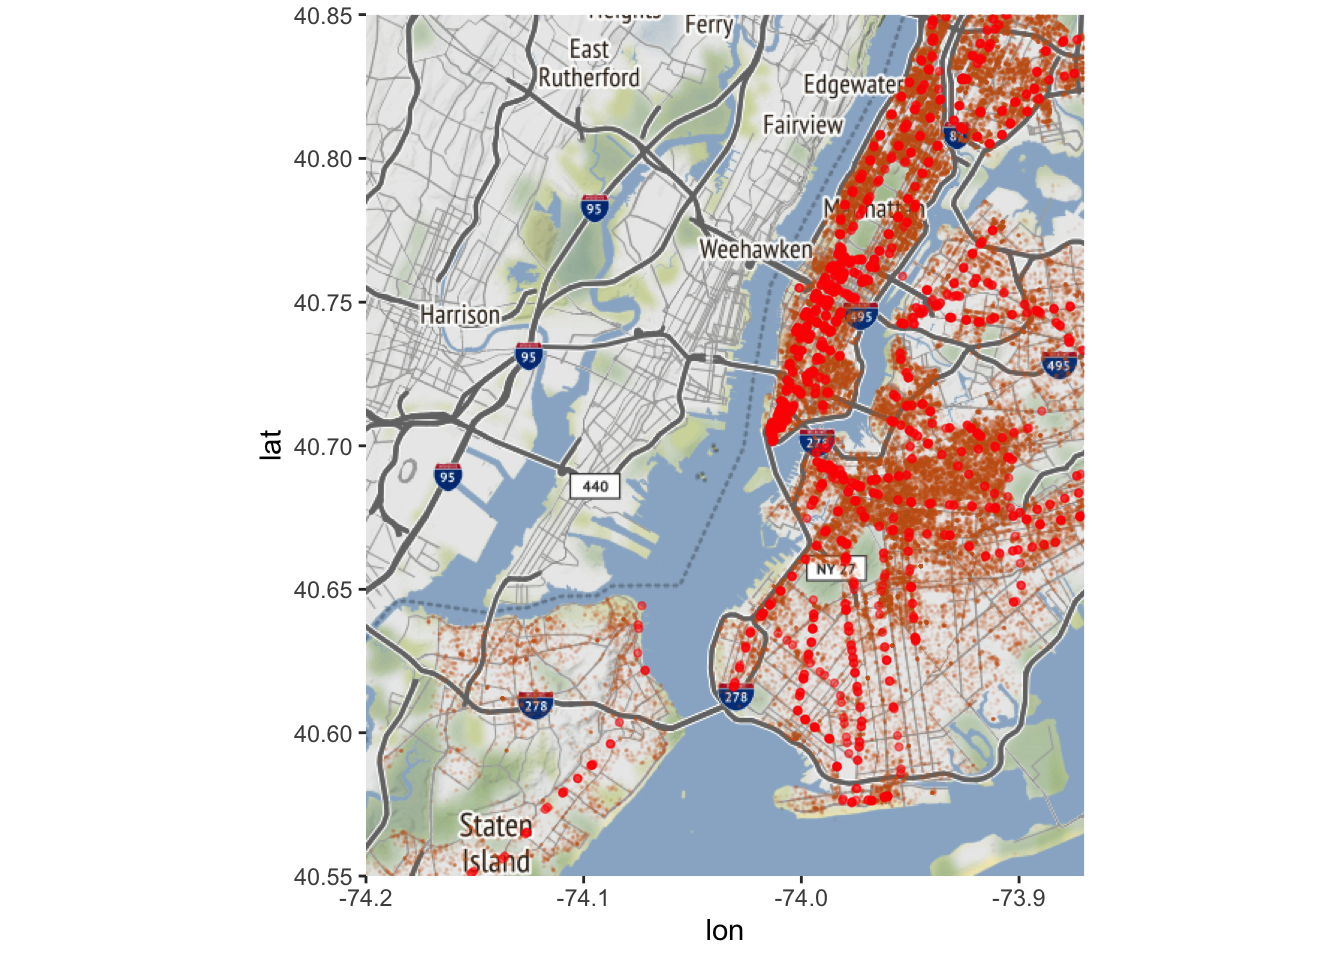
\includegraphics{Rats-PreAnalysis_files/figure-latex/unnamed-chunk-5-1.pdf}

\begin{Shaded}
\begin{Highlighting}[]
\CommentTok{\# system.time(\{}
\CommentTok{\# minSubwayDist = function(longitude, latitude)}
\CommentTok{\# \{}
\CommentTok{\#   min =  as.integer(.Machine$integer.max)}
\CommentTok{\#   for (i in (1:nrow(subway\_entrances)))}
\CommentTok{\#   \{}
\CommentTok{\#     distance = distm(c(longitude, latitude), c(longs[i], lats[i]), fun = distHaversine)[1]}
\CommentTok{\#     if(distance\textless{}min)}
\CommentTok{\#     \{}
\CommentTok{\#       min=distance}
\CommentTok{\#     \}}
\CommentTok{\#   \}}
\CommentTok{\#   return(min)}
\CommentTok{\# \}}
\CommentTok{\# }
\CommentTok{\# ratSubsetM \textless{}{-} ratSubsetM \%\textgreater{}\% drop\_na(Longitude)}
\CommentTok{\# ratSubsetM \textless{}{-} ratSubsetM \%\textgreater{}\% drop\_na(Latitude)}
\CommentTok{\# \# ratsub = rats[1:100,]}
\CommentTok{\# ratSubsetM \textless{}{-} ratSubsetM \%\textgreater{}\% add\_column(minSubwayDistance = NA)}
\CommentTok{\# }
\CommentTok{\# mindists = 1:nrow(ratSubsetM)}
\CommentTok{\# for(i in (1:nrow(ratSubsetM)))}
\CommentTok{\# \{}
\CommentTok{\#   mindists[i] = minSubwayDist(ratSubsetM$Longitude[i], ratSubsetM$Latitude[i])}
\CommentTok{\# \}}
\CommentTok{\# ratSubsetM$minSubwayDistance = mindists}
\CommentTok{\# \})}
\end{Highlighting}
\end{Shaded}

\begin{Shaded}
\begin{Highlighting}[]
\CommentTok{\#I want to now do a correlation between "region" and (rat count/area of region). nyc\_neighborhoods\_df is stored in the same way as states are in HW09.}

\CommentTok{\#should also do proportion of "bad restaurants" to "good restaurants" per region}
\end{Highlighting}
\end{Shaded}


\end{document}
